\documentclass[UTF8]{ctexbook}

\usepackage[titles]{tocloft} % 目录
\usepackage[colorlinks,linkcolor=blue]{hyperref}
% \usepackage{graphicx} % An example of a floating figure using the graphicx package.
\usepackage{animate}
\usepackage{enumerate}

\renewcommand\thesection{\arabic{section}}
% arabic 阿拉伯数字 roman 小写的罗马数字 Roman 大写的罗马数字 alph 小写字母  Alph 大写字母
\begin{document}
% ----------- 封面 ---------------
\begin{center}  % 居中
	\quad \\
	\vspace{3cm}
	\hspace{3cm}\Huge{A NOTE of MASTER}\\
	\hspace{3cm}\Huge{菜鸟硕士手册} \\
	\hspace{3cm}\large{V1.0} \\
	\vspace{5cm}
	\hspace{3cm}\href{https://github.com/lonelybag/Latex_lonelybag}{\Large{@LonelyBag}}\\
	\vspace{0.5cm}
	\hspace{3cm}\Large {2018.3.2}
	\clearpage  % 清除当页页码
\end{center}

\thispagestyle{empty}
\clearpage  % 清除当页页码
% ----------- 目录 ---------------
\tableofcontents
\clearpage
\newpage
\quad
\newpage
\clearpage
% ----------- 正文 ---------------
\section{快速抓住研究热点}
研究热度往往体现在论文的发表数量中,但是一个领域中的主要研究方向却往往很难仅通过阅读论文而获得全面认识。换句话说,统计论文中的研究方向远比统计发表数量重要。为了解决这一问题,研究人员也提出了若干解决方案。

\subsection{传统方式}
词典,是语言学家针对特定语言而将常见字词按照一定的逻辑编纂起来的文本工具。科学家也有自己的词典,他们针对某一特定研究领域对热点论文进行总结归纳并提出相应见解,最终以论文的形式发表,这就是文献综述。

通过阅读文献综述,可以快速地对所关注的研究领域形成大致了解,而这也是快速抓住研究热点的传统方式。通过限定检索词可以较为有效地检索该类型的文章,对于英文文献,其检索词可以选择如下几种:
\begin{itemize}
	\item Review
	\item Challenge
	\item Survey
	\item Statement
	\item ... ...
\end{itemize}

这样,再加上一些限定词(如:WPT)就可以有效地检索出特定研究领域的文献综述。但是,这样检索出的文献往往比较松散,并且会使我们忽略一些更有价值的paper。因此,有时(甚至往往)会采用辅助工具进行这项工作。

\subsection{辅助工具}
为了快速地了解一个领域的研究热点,仅仅通过 {\bf 关键词检索 - 论文下载 - 阅读 - 二次检索} 这类流程是不能达到“快速”的要求的,真正有效的方法是借助论文分析工具,这类工具一般有如下特点:

\begin{itemize}
	\item 可以分析大量文献间的交叉检索关系
	\item 结果可视化
	\item 多功能
\end{itemize}

常用的辅助工具有:\href{https://zhuanlan.zhihu.com/p/20902898}{HistCite Pro 2.1} 以及 \href{https://zhuanlan.zhihu.com/p/30970993}{VOSviewer}。这两种工具的最大区别就是HistCite Pro 2.1仅支持英文文献,但VOSviewer不仅支持英文还支持中国知网导出的中文文献。笔者只用过HistCite Pro 2.1,如果读者希望对中文文献也进行处理,可以参考\href{https://www.jianshu.com/p/e20f3f1d17d8}{这个})。下面我通过若干gif对软件的使用进行介绍。
\subsubsection{安装}
安装就不赘述了,参考\href{https://zhuanlan.zhihu.com/p/20902898}{这里}就够了。
\subsubsection{导出文献}
这一步是初学者最容易出现差错的地方,这是因为HistCite Pro 2.1对源数据的格式要求非常严谨,而且它仅支持由Web of Science导出的文献格式。下面我通过Step-by-step的方式展示如何从WOS导出符合要求的格式。

第一步:选择检索{\bf 数据库}并给定检索词,一般首次使用需要我们对整个领域有一个宏观认识,因此检索词可以非常概括,比如我使用的wireless power,如图\ref{fig:1}。

\begin{figure}[!htb]
	\centering
	\animategraphics[autoplay, loop , width=0.9\linewidth]{8}{Figure//WOSsearch//10}{01}{80}
	\vspace{-0.3cm}
	\caption{WOS检索关键词:wireless power}\label{fig:1}
\end{figure}

第二步:选择正确格式,下载,如图\ref{fig:2}所示。值得注意的是,WOS仅支持一次性导出500篇文献,所以更多的文献需要多次下载。

\begin{figure}[!htb]
	\centering
	\animategraphics[autoplay, loop , width=0.9\linewidth]{8}{Figure//WOSdownload//00}{01}{98}
	\vspace{-0.3cm}
	\caption{WOS下载特定格式检索结果}\label{fig:2}
\end{figure}

第三步,需要将下载获得的所有txt移动至TXT文件夹,然后打开main.exe,此时输入1并回车,软件将自动打开程序界面,接着点击gragh maker,我们就会获得文献之间的引用网络,文献由节点表示,所有的节点自上而下按照时间顺序排列,之间的引用和被引关系由连接的线条表示。修改count将对分析的文献数量进行控制,一般来说,取得大一点可以获得更多的信息,如图\ref{fig:3}所示。

\begin{figure}[!htb]
	\centering
	\animategraphics[autoplay, loop , width=0.9\linewidth]{8}{Figure//Hmaker//00}{01}{73}
	\vspace{-0.3cm}
	\caption{HistCite Pro 2.1操作}\label{fig:3}
\end{figure}


注意到,select by一栏有两个选项:LCS和GCS,LCS是Local Citation Score的缩写,代表某篇文献在本地数据集(也就是我们所下载的txt集合)的总被引次数,而GCS是Global Citation Score的缩写,代表在WOS数据库中的总被引次数。一般来说,由于本地数据集是根据我们的关键词获得的,因此LCS排名更能够反映某一学科的发展。此外,还有两个参数会出现在浏览器界面,CR和LCR,分别是Cited references和local cited references的缩写,代表对WOS数据库和本地数据库文献引用的数量。这里,CR越高(一般以50篇为标准)则表示该文献越可能是综述性文献,这样就可以方便地追根溯源,清晰地看到一个学科乃至一个领域的发展脉络,一个典型的发展脉络可以参考图\ref{fig:typical_trace}(完整版请\href{https://raw.githubusercontent.com/lonelybag/Latex_lonelybag/V1.0/Script/002_NOTE_of_MASTER/Figure/typical_trace_full.jpg}{移步})。

\begin{figure}[!htb]
	\centering
	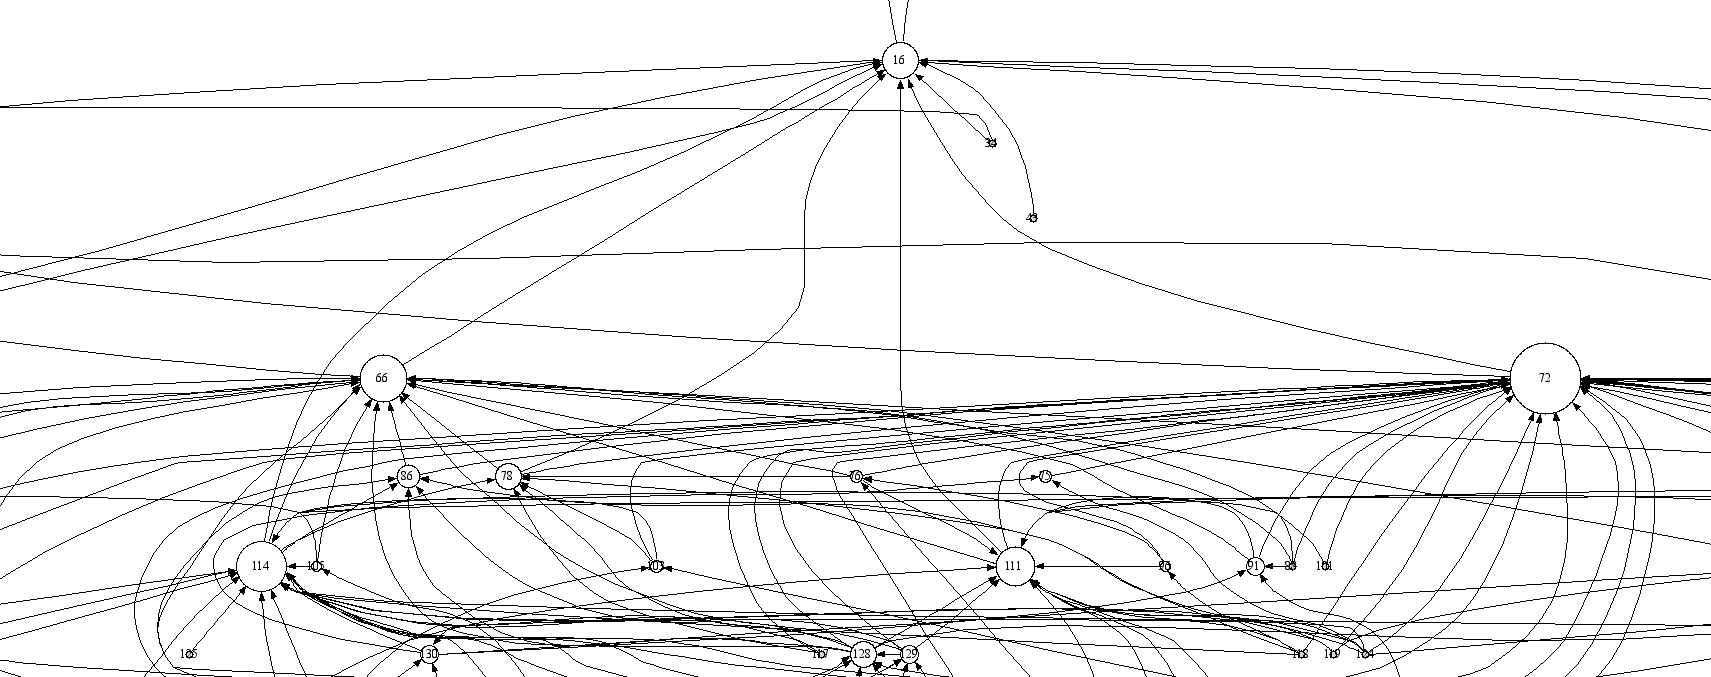
\includegraphics[width=1\linewidth]{Figure/typical_trace.JPG}
	\vspace{-0.3cm}
	\caption{一个示例}\label{fig:typical_trace}
\end{figure}

可以看出,文献16显然是这个领域的开创性论文,随着时间的推移又分裂为两个分支,接着又发展为多个分支。通过阅读关键节点论文不仅可以快速了解这个领域的发展脉络,甚至还可以看出:

\begin{itemize}
	\item 研究之初,两个小方向是经过试探却又半途而废的
	\item \href{https://raw.githubusercontent.com/lonelybag/Latex_lonelybag/V1.0/Script/002_NOTE_of_MASTER/Figure/typical_trace_full.jpg}{完整版图片}右侧出现了两个领域的交叉,这里往往是研究思路的“不老泉”
	\item \href{https://raw.githubusercontent.com/lonelybag/Latex_lonelybag/V1.0/Script/002_NOTE_of_MASTER/Figure/typical_trace_full.jpg}{完整版图片}最左侧有一个研究历程非常持久的小分支,这可能是某个专家的“独门秘籍”
	\item \href{https://raw.githubusercontent.com/lonelybag/Latex_lonelybag/V1.0/Script/002_NOTE_of_MASTER/Figure/typical_trace_full.jpg}{完整版图片}右侧还有一个完全没有关联的领域,虽然在2013年后就没有产出了,但是这并不一定意味着研究的停滞,也有可能是研究成果实现了产业化,被大佬们拿去挣钱了。。。
	\item 。。。 。。。
\end{itemize}

所以,这个方法不仅仅可以帮助我们找文献,更重要的是带给了我们关于这项研究的历史发展历程,带给了我们冰冷研究的人文情怀,我们甚至可以想象出,那位开山鼻祖级别的大佬在当时仅仅是一位年轻博士生的时候的艰苦、悲痛、遇到机遇时狂喜、受挫后的再一次站立、以及功成名就之后的平凡和悠闲。。。

因此,每一张图都可以说是一位科学家的成名史、一个领域的发展史、以及整个人类文明的历史。

所以,为什么不试试\href{https://zhuanlan.zhihu.com/p/20902898}{它}或\href{https://zhuanlan.zhihu.com/p/30970993}{它}呢?

\section{常用网站}


\section{COMSOL}

\section{基本}
\subsection{杀毒+垃圾整理+系统优化}
\begin{itemize}
	\item \underline{\textit{\href{https://www.huorong.cn}{火绒}}}\quad 免费
	\item \underline{\textit{\href{http://ccleaner.soft88.com}{ccleaner}}}\quad 基础版免费
	\item \href{https://bitsum.com}{Process Lasso}\quad 用于优化系统进程,提高运行速度,收费
	\item \href{https://fastcopy.jp/en/}{FastCopy}\quad 文件复制加速软件,免费
	\item \underline{\textit{\href{https://www.listary.com}{Listery}}}\quad 用于快速搜索文件,免费
	\item \href{http://www.disktool.cn/download.html}{傲梅分区助手}\quad 用于分区,免费
	\item \underline{\textit{\href{http://www.bandisoft.com}{Bandizip}}}\quad 据说是第二好用的压缩软件,免费
\end{itemize}

\subsection{卸载类}
\begin{itemize}
	\item \href{https://geekuninstaller.com}{Geek}\quad 免费
	\item \underline{\textit{\href{https://www.revouninstaller.com/}{Revo Uninstaller Pro}}}\quad 收费
	\item \underline{\textit{\href{https://lockhunter.com}{lockhunter}}}\quad 用于删除时出现该文件正在占用,3M,免费
	\item
\end{itemize}

\subsection{下载}
\begin{itemize}
	\item \href{http://jdownloader.org/jdownloader2}{JDownloader2}
	\item \href{http://xdman.sourceforge.net}{Xtreme Download Manager}\quad 36M,免费
	\item \href{https://www.freedownloadmanager.org/}{FDM}\quad 48.7M,免费
	\item \href{https://webtorrent.io}{磁力在线播放}
	\item \href{https://send-anywhere.com}{Send Anywhere}\quad 设备之间的分享
	\item 百度网盘满速下载,微信关注 科研利器
\end{itemize}

\subsection{制作文档类}
\begin{itemize}
	\item GIF录屏:\underline{\textit{\href{https://www.cockos.com/licecap/}{LICEcap}}}\quad 230kb免费、\href{https://www.screentogif.com/?l=zh_cn}{ScreenToGif}\quad 2M免费、\href{https://ocam.en.softonic.com}{Ocam}\quad 10Mb免费
	\item Gif转换为图片:\underline{\textit{\href{https://ulead-gif-animator.jaleco.com}{Ulead GIF Animator}}}\quad 免费
	\item PDF转换为矢量图片:\underline{\textit{\href{https://inkscape.org}{Inkscape}}}\quad 免费
	\item \underline{\textit{\href{https://code.visualstudio.com}{VScode}}}\quad 免费
	\item \underline{\textit{\href{https://mirrors.tuna.tsinghua.edu.cn/CTAN/systems/texlive/Images/}{Texlive}}}\quad 免费
	\item 截屏:\underline{\textit{\href{http://www.faststone.org/FSCaptureDetail.htm}{FastStone Capture}}}\quad 收费、\href{https://www.snipaste.com}{Snipaste}\quad 免费
	\item 快速浏览:\href{https://pooi.moe/QuickLook/}{QuickLook}\quad 免费、\href{http://1218.io}{seer}\quad 收费
	\item \href{https://otp.landian.vip/zh-cn/}{office365}
	\item \href{http://www.dayanzai.me/infixpro-pdf-editor.html}{InfixPro PDF Editor}\quad 修改PDF
\end{itemize}

\subsection{Chrome插件类}
\begin{itemize}
	\item \underline{\textit{\href{https://greasyfork.org/zh-CN}{油猴脚本}}}\quad 免费
	\item VPN:就去加速(官网已被墙)
	\item \underline{\textit{\href{http://listen1.github.io/listen1/}{Listen1}}}\quad 最好用的在线音乐播放器,免费
	\item \href{https://kopernio.com}{Kopernio}\quad 免费获取论文,免费
\end{itemize}

\subsection{常用网站}
\begin{itemize}
	\item 软件下载
	      \begin{itemize}
		      \item \href{https://www.3d66.com/popsoft_26.html}{软件下载}\quad 包括但不限于:3DSMAX,AutoCAD,PS,Rhino,Maya,AI。。。
		      \item \href{https://www.appinn.com/category/windows/}{小众软件}
		      \item \href{https://filehippo.com/zh/}{国际类软件网站}
	      \end{itemize}
	\item Git
	      \begin{itemize}
		      \item \href{http://gitbook.liuhui998.com/index.html}{gitbook}
		      \item \href{https://learngitbranching.js.org/?demo}{动画学习Git}
	      \end{itemize}
	\item 在线工具
	      \begin{itemize}
		      \item \href{https://tool.lu}{程序员的工具箱}
		      \item \href{https://cloudconvert.com/gif-to-mp4}{Gif2MP4}
		      \item \href{https://cn.office-converter.com/FIG-to-EPS}{Fig2EPS}
		      \item \href{http://www.ytube.win}{下载youtube视频}\quad 缺点是不带字幕
		      \item \href{https://www.slant.co}{帮助我们做决策}
		      \item \href{https://www.photopea.com}{在线PS}
		      \item \href{https://uzer.me/u/signin}{在线office,PS,AI,MATLAB等}
		      \item \href{https://bigjpg.com}{无损放大图片}
		      \item \href{https://www.remove.bg}{自动抠图}
	      \end{itemize}
	\item 在线学习
	      \begin{itemize}
		      \item \href{http://www.xuexiniu.com/forum.php?mod=forumdisplay&fid=102&filter=typeid&typeid=1}{犀牛技巧}
		      \item \href{http://www.pythontutor.com}{python代码在内存中是如何执行的}
		      \item \href{https://algorithm-visualizer.org}{算法运行可视化}
	      \end{itemize}
\end{itemize}

\section{论文写作}
\subsection{制作文档类}
\begin{itemize}
	\item \underline{\textit{\href{https://mirrors.tuna.tsinghua.edu.cn/CTAN/systems/texlive/Images/}{Texlive}}}\quad 免费
	\item 思维导图:\href{https://mubu.com}{幕布}\quad 34Mb,免费
	\item 截屏:\underline{\textit{\href{http://www.faststone.org/FSCaptureDetail.htm}{FastStone Capture}}}\quad 收费、\href{https://www.snipaste.com}{Snipaste}\quad 免费
	\item \href{https://picpick.app/zh/}{PicPickp}\quad 屏幕取色
	\item \href{https://ditto-cp.sourceforge.io}{Ditto}\quad 剪切板神器,免费
	\item 批量更改文件名:\underline{\textit{\href{http://www.ffhome.com/works/1406.html}{菲菲更名宝贝}}}\quad 名字奇怪,但是好用
\end{itemize}

\subsection{Chrome插件类}
\begin{itemize}
	\item \href{https://kopernio.com}{Kopernio}\quad 免费获取论文,免费
\end{itemize}

\subsection{英语写作}
\begin{itemize}
	\item 英语语法检查 \href{https://languagetool.org}{LanguageTool}、\underline{\textit{\href{https://www.grammarcheck.net}{grammercheck}}}、\href{https://www.scribens.com}{scribens}、\href{https://www.grammarly.com}{grammerly}、\href{https://www.nounplus.net}{nounplus}
	\item 查单词搭配等等 \underline{\textit{\href{https://www.english-corpora.org/coca/}{ Corpus of Contemporary American English}}}、\href{https://www.lintcode.com}{linggle}
	\item 近义词 \underline{\textit{\href{https://www.thesaurus.com}{theasurus}}}
\end{itemize}

\subsection{科研常用网站}
\begin{itemize}
	\item 文献写作
	      \begin{itemize}
		      \item \href{http://www.latexstudio.net/archives/6888.html}{GB/T7714-2015参考文献格式}\quad 毕业论文参考文献,自动生成
		      \item \href{https://www.processon.com/login;jsessionid=022BCDCA031DD3C240BE7FD87D942F03.jvm1?backUrl=/diagraming/5be7a513e4b0d74dc539976e}{流程图}
		      \item Latex相关:
		            \begin{itemize}
			            \item \href{http://detexify.kirelabs.org/classify.html}{手写LaTeX符号}
			            \item \href{http://www.jabref.org}{JabRef}\quad 开源的文献管理软件
			            \item \href{http://www.latexstudio.net/archives/6992.html}{Excel2Latex}
			            \item \href{http://www.ursoswald.ch/metapost/introduction.html}{MetaPOST}\quad 矢量绘图软件
			            \item \href{http://www.gnuplot.info}{Gnuplot}\quad 绘制矢量数据图
			            \item \href{https://www.tablesgenerator.com/#}{在线绘制表格}
			            \item \href{http://math.ecnu.edu.cn/~jypan/Teaching/Latex/}{LaTeX 科技排版}
			            \item \href{http://www.latexstudio.net/}{latex开源小屋}
			            \item \href{https://github.com/latexstudio}{Latex中文社区Github}
			            \item \href{https://www.overleaf.com/login}{在线编辑器1}、\href{http://www.math.org.cn/tex/index.html}{在线编辑器2}
			            \item \href{http://www.bakoma-tex.com}{一个我认为完美的编辑器}\quad 缺点:收费
		            \end{itemize}
	      \end{itemize}
	\item 绘图
	      \begin{itemize}
		      \item \href{https://www.photopea.com}{在线PS}
		      \item \href{https://uzer.me/u/signin}{在线office,PS,AI,MATLAB等}
		      \item \href{https://bigjpg.com}{无损放大图片}
		      \item \href{https://www.remove.bg}{自动抠图}
		      \item 思维导图:\href{http://naotu.baidu.com/file/97d9cd5ca30672903a3e3321e62c6ed8}{百度脑图}、\href{https://www.xmind.net/}{Xmind}
		      \item \href{http://www.colorhunter.com}{Color Hunter}\quad 配色
		      \item \href{https://color.adobe.com/zh/create/color-wheel/?base=2&rule=Analogous&selected=0&name=我的%20Color%20主題&mode=rgb&rgbvalues=1,0.8549019607843137,0.598371339694025,0.91,0.33228399543185755,0.04550000000000004,1,0,0,0.8452221384131547,0.04550000000000004,0.91,0.3394492552539419,0.050000000000000044,1&swatchOrder=0,1,2,3,4}{Adobe Color CC}
		      \item
	      \end{itemize}
	\item 学习类
	      \begin{itemize}
		      \item \href{https://www.52pojie.cn/thread-716675-1-1.html}{一个电路仿真APP}\quad 特点是,可以看到电流
		      \item \href{https://mm.edrawsoft.cn/map.html?obj=wxoa3v5wBLcpmgCifx59_Uzk5X4qHU/Personal/未命名文件.emmx}{思维导图}更专业一点
		      \item \href{https://ankiweb.net/shared/decks/}{记忆神器}
	      \end{itemize}
	\item 算法以及神经网络
	      \begin{itemize}
		      \item \href{https://leetcode.com}{Leetcode}以及\href{https://www.lintcode.com/zh-cn/accounts/signup/}{lintcode} 代码训练平台
		      \item \href{https://algorithm-visualizer.org}{算法运行可视化}
		      \item \href{https://www.stateoftheart.ai}{MIT整理的关于神经网络的论文}
		      \item \href{https://github.com/lonelybag/pwc}{神经网络论文以及源代码}\quad 万能的GitHub
	      \end{itemize}
\end{itemize}

\subsection{绘图}
\begin{itemize}
	\item 电路图
	      \begin{itemize}
		      \item Viso
		      \item Latex
		      \item Python
		      \item
	      \end{itemize}
	\item 流程图:
	      \begin{itemize}
		      \item
	      \end{itemize}
	\item 统计数据函数图:
	      \begin{itemize}
		      \item Origin
		      \item Sigmaplot
		      \item Graphpad
		      \item geogebra(开源)
		      \item SPSS
		      \item NVivo
	      \end{itemize}
	\item 2D 图形
	      \begin{itemize}
		      \item Photoshop
		      \item Adobe Illustrator
		      \item \href{https://affinity.serif.com/zh-cn/designer/}{affinity designer}
	      \end{itemize}
	\item 3D 拟物图
	      \begin{itemize}
		      \item C4D
		      \item 3ds MAX
	      \end{itemize}
\end{itemize}

\section{其他}
\begin{itemize}
	\item Send Anywhere
	\item \href{https://www.scimagojr.com}{SCI期刊}
	\item \href{http://libgen.io}{免费专业书籍}
\end{itemize}

\section{最小配置}
在此给出一个我常用的\emph{最小基础配置}:
\begin{itemize}
	\item 杀毒软件:\href{https://www.huorong.cn}{火绒}
	\item 卸载软件:\href{http://www.xue51.com/soft/11977.html}{Revo Uninstaller Pro}
	\item 文档撰写:\href{https://mirrors.tuna.tsinghua.edu.cn/CTAN/systems/texlive/Images/}{\LaTeX} 和 WORD
	\item PDF阅读:\href{https://www.tracker-software.com/product/pdf-xchange-editor}{PDF-XChange Editor}
	\item 视频播放:\href{http://potplayer.daum.net/?lang=zh_CN}{PotPlayer}
	\item 文件搜索:\href{https://www.listary.com}{Listery}
	\item 撸代码: \href{https://code.visualstudio.com}{VScode}
	\item 版本管理+团队协作:\href{https://git-scm.com}{Git}
\end{itemize}

\emph{最小科研配置}:
\begin{itemize}
	\item 计算与仿真:
	      \begin{itemize}
		      \item 数值计算:Matlab、Mathematica
		      \item 电路仿真:ADS、Simulink
		      \item 电磁场仿真:Comsol
	      \end{itemize}
	\item 文档撰写:
	      \begin{itemize}
		      \item Latex
		      \item Endnote
		      \item \href{https://zhuanlan.zhihu.com/p/20902898}{HistCite Pro 2.1}
	      \end{itemize}
\end{itemize}



\backmatter
\chapter{跋}
讲几个事例作为结束。

\subsection*{热爱}
时常有人问我:“你怎么会有时间去学那么多东西的?”。其实很简单,因为热爱。

\subsection*{持久的输出}
知乎上有一个问题,苹果公司有哪些黑科技?其中一个回答的答案是iPhone一代。2007年1月,苹果公司发布了被后人称为“重新定义了手机”的iPhone一代,自此开始了长达十年的封神之路。作为历史上市值第一个超过万亿美元的科技公司,它的成功也让很多人萌发了试图复制这一商业成功的欲望,当然他们并未成功,因为十年后的今天苹果依然是第一。很多人将苹果的成功归功于乔布斯,这种想法其实很愚蠢。那么到底是什么造就了它的成功呢?

如果大家读过《乔布斯传》就会了解到,2007年发布的iphone一代,其实早在5年前就已经开始准备了。那就是2002年,还是各种翻盖、滑盖、旋转盖手机迭起的风云时代。。。

我们输的不冤枉。对手感觉到的“黑科技”,其实对自己不过是孕育和必然。

\subsection*{人为什么活着?}
为了心中的梦想。

\vspace{2cm}
总结起来就是三句话:试着让内心去做决策,时刻雕琢自己以及捍卫梦想。

\hspace{4cm}\\
\noindent2019毕业前夕\\
于天津工业大学 \quad 电气学院






\appendix
\chapter{附录 A}\label{fuluA}
如果大家看过《降临》这部电影就会了解,语言决定了(或者反映了)一个人的思考方式,电影中的外星人具有非线性的高维语言能力,没有时间空间的线性概念,这也是电影中人类语言学家不能理解外星人文字的症结。我们可以仿照着看一下汉语与英语的差别,如表\ref{tab:compareCandE}:

\begin{table}[!htb]
	\renewcommand{\arraystretch}{1.3} %可以让行显得更加宽敞
	\caption{中英对比}\label{tab:compareCandE}
	\centering
	\animategraphics[autoplay, loop , width=0.6\linewidth]{8}{Figure//Fig2//10}{01}{19}
	\vspace{-0.3cm}
	\caption{This is an awesome pdf with a gif - by lonelybag.}\label{fig:39}
\end{figure}

\section{文献写作}
\subsection{写作工具}
\subsection{写作流程}
\subsection{参考文献}

\end{document}
